\documentclass[11pt]{article}
\usepackage[scaled=0.92]{helvet}
\usepackage{geometry}
\geometry{letterpaper,tmargin=1in,bmargin=1in,lmargin=1in,rmargin=1in}
\usepackage[parfill]{parskip} % Activate to begin paragraphs with an empty line rather than an indent %\usepackage{graphicx}
\usepackage{amsmath,amssymb, mathrsfs, dsfont}
\usepackage{mathtools}

\usepackage{tabularx}
\usepackage[font=footnotesize,labelfont=bf]{caption}
\usepackage{graphicx}
\usepackage{xcolor}
%\usepackage[linkbordercolor ={1 1 1} ]{hyperref}
%\usepackage[sf]{titlesec}
\usepackage{natbib}
\usepackage{../../Tianpei_Report}

%\usepackage{appendix}
%\usepackage{algorithm}
%\usepackage{algorithmic}

%\renewcommand{\algorithmicrequire}{\textbf{Input:}}
%\renewcommand{\algorithmicensure}{\textbf{Output:}}



\begin{document}
\title{Lecture 7: Planning and Learning with Tabular Methods}
\author{Tianpei Xie}
\date{ Aug 8th., 2022 }
\maketitle
\tableofcontents
\newpage
\section{Introduction}
There is a unified view of reinforcement learning methods:
\begin{itemize}
\item \emph{\textbf{model-based}} reinforcement learning methods: Model-based methods rely on \emph{\textbf{planning}} as their primary component. Examples include the \emph{dynamic programming} methods and the \emph{heuristic search} such as $A^*$.

\item \emph{\textbf{model-free}} reinforcement learning methods: Model-free methods primarily rely on \emph{\textbf{learning}}. Examples include \emph{Monte Carlo methods} and \emph{temporal difference (TD) methods}. 
\end{itemize}
The heart of both kinds of methods is the \underline{computation of value functions}. Moreover, all the methods are based on looking ahead to future events, computing a \emph{backed-up} value, and then using it as an update target for an \emph{approximate} value function.

\begin{figure}
\begin{minipage}[t]{1\linewidth}
  \centering
  \centerline{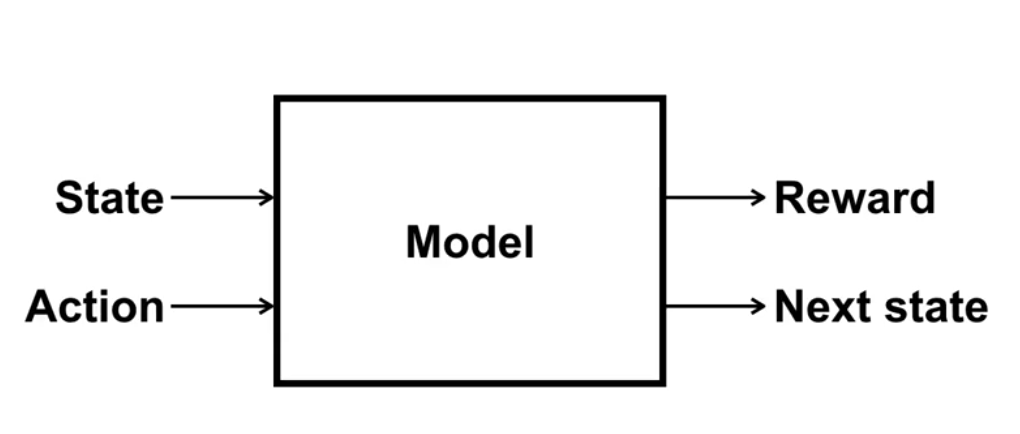
\includegraphics[scale = 0.3]{model_rl.png}}
\end{minipage}
\caption{\footnotesize{\textbf{A model in  reinforcement learning}}}
\label{fig: tabluar_methods_diagram}
\end{figure}
\section{Models and Planning}
By a \emph{model} of the environment we mean anything that an agent can use to predict how the environment will respond to its actions. Given a state and an action, a model produces a prediction of the resultant next state and next reward.

There are two type of models:
\begin{itemize}
\item \emph{\textbf{distribution models}}: models produce a description of \emph{all possible} next-state-reward pairs and their probabilities. Dynamic Programming algorithms assume distribution models, since we need to know probability $p(s', r| s, a)$ for all next-state-reward pairs $s', r$ given every state $s$ and action $a$. Distribution models are \emph{stronger} than sample models in that they can always be used to produce samples. 

A typical class of distribution models is the \textbf{\emph{Probabilistic Graphical Model}} \citep{koller2009probabilistic} including the \emph{Bayesian Networks}, \emph{Markov Networks}, \emph{Gaussian  Graphical Models}, etc. These models use graph representation to \emph{factorize} the global joint distribution between states, actions and rewards into several connected local factors embedded in subgraphs. 


\item \emph{\textbf{sample models}}:  models produce just one of the possibilities, \emph{sampled} according to the probabilities. Sample models can be sampling algorithms such as \emph{importance sampling}, sequential sampling like \emph{Markov Chain Monte Carlo}, \emph{Gibbs sampling}, or \emph{Gradient Flow methods} etc.
\end{itemize}
Note that model is used to \underline{\emph{simulate}} the environment and produce \underline{\emph{simulated experience}}. This is in contrast to the actual environment which generates the  \underline{\emph{real experience}}. The word \textbf{\emph{planning}} is used in several different ways in different fields. We use the term to refer to any computational process that takes a model as input and produces or improves a policy for interacting with the modeled environment. (Figure \ref{fig: planning})

\begin{figure}
\begin{minipage}[t]{1\linewidth}
  \centering
  \centerline{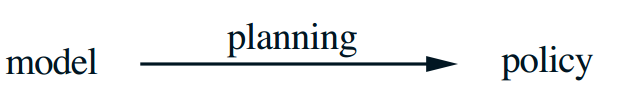
\includegraphics[scale = 0.3]{planning.png}}
\end{minipage}
\caption{\footnotesize{\textbf{Planning}}}
\label{fig: planning}
\end{figure}

Given probabilistic models, one can use \textbf{sampling methods} \citep{liu2001monte} such as \emph{Importance Sampling},  \emph{Markov Chain Monte Carlo (MCMC)} such as \emph{Gibs sampling}, \emph{Metropolis Algorithm} etc to obtains samples of actions and states. 


There are two type of planning:
\begin{itemize}
\item \underline{\emph{\textbf{State-space planning}}} is viewed primarily as a search through the \emph{state space} for an \emph{optimal policy} or an optimal path to a goal. Actions cause transitions from state to state, and value functions are computed over states. In \emph{reinforcement learning}, we mainly concerned about state-space planning. 

\item \emph{\textbf{Plan-space planning}}, planning is instead a search through the space of plans. Operators transform one plan into another, and value functions, if any, are defined over the space of plans. Example includes \textbf{evolutionary algorithm} and \textbf{genetic algorithm}.  Plan-space methods are difficult to apply efficiently to the stochastic sequential decision problems that are the focus in reinforcement learning.
\end{itemize}

All state-space planning methods discussed here share a common structure : there are two basic ideas: (1) all state-space planning methods involve \textbf{computing value functions} as a key intermediate step toward \textbf{improving the policy}, and (2) they compute value functions by \underline{updates} or \underline{backup} operations applied to \textbf{simulated experience}. This common structure can be diagrammed as follows: (Figure \ref{fig: state_space_planning})

\begin{figure}
\begin{minipage}[t]{1\linewidth}
  \centering
  \centerline{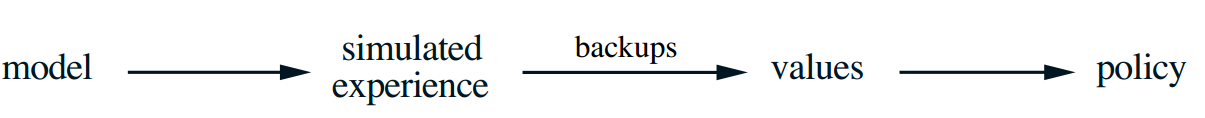
\includegraphics[scale = 0.3]{state-space_planning.png}}
\end{minipage}
\caption{\footnotesize{\textbf{state-space planning structure}}}
\label{fig: state_space_planning}
\end{figure}

The heart of both \emph{learning} and \emph{planning} methods is the \textbf{estimation of value functions} by \underline{backing-up update} operations.  The
difference is that whereas planning uses \emph{simulated experience} generated by a model, learning methods use \emph{real experience} generated by the environment. In particular, in many cases a learning algorithm can be \emph{substituted} for the key update step of a planning method. 

Figure \ref{fig: tabular_q_planning} shows the \emph{\textbf{random-sample one-step tabular Q-planning}}, converges to the optimal policy for the model under the same conditions that one-step tabular Q-learning converges to the optimal policy for the real environment. Compared to the Q-learning, we need that the only difference is that the samples used to update the Q function is generated by the model. Also the starting state and actions are selected at random. 
\begin{figure}
\begin{minipage}[t]{1\linewidth}
  \centering
  \centerline{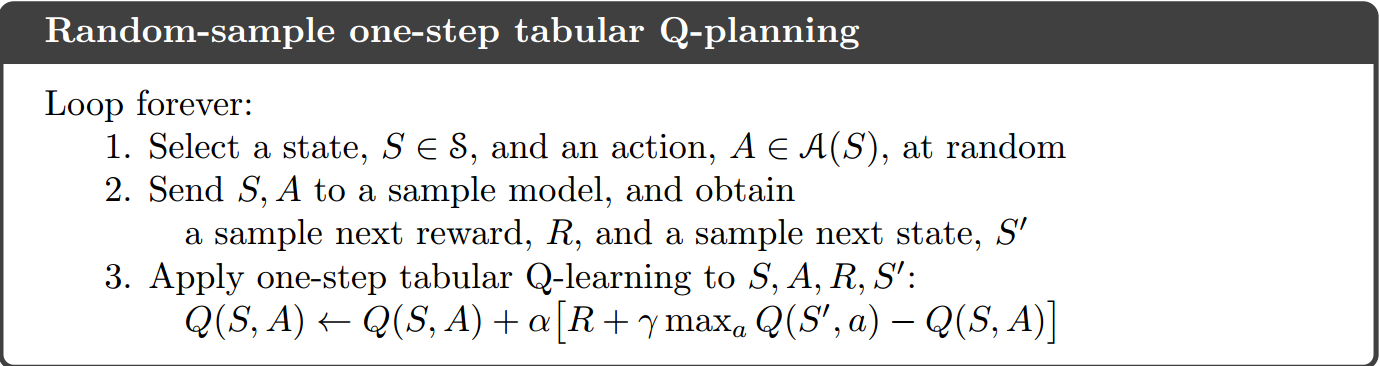
\includegraphics[scale = 0.3]{tabular_q_planning.png}}
\end{minipage}
\caption{\footnotesize{\textbf{Tabular Q-planning}}}
\label{fig: tabular_q_planning}
\end{figure}

\section{Dyna: Integrated Planning, Acting, and Learning}
When planning is done online, while interacting with the environment, a number of interesting issues arise. New information gained from the interaction may change the
model and thereby interact with planning. It may be desirable to customize the planning process in some way to the states or decisions currently under consideration, or expected in the near future. If decision making and model learning are both computation-intensive processes, then the available computational resources may need to be divided between them.

\begin{figure}
\begin{minipage}[t]{1\linewidth}
  \centering
  \centerline{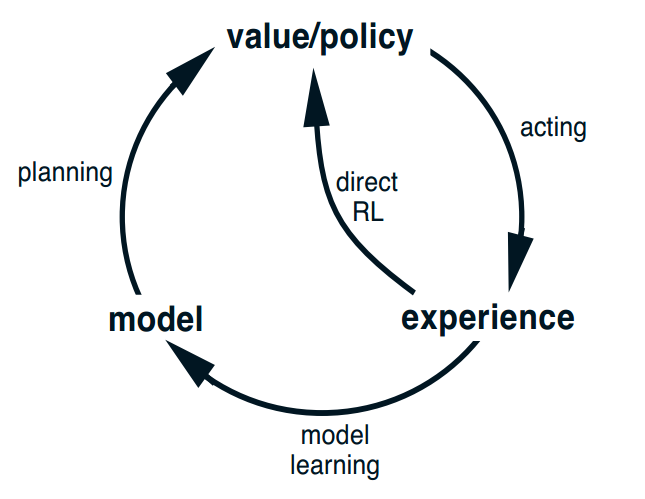
\includegraphics[scale = 0.3]{Planning_learning_relationship.png}}
\end{minipage}
\caption{\footnotesize{\textbf{The generic relationship between model learning, direct RL, planning in a planning agent. Note that the value/policy can be updated either by real experience via direct RL or by simulated experience via planning. Meanwhile, the real experience will be used for model update/learning. }}}
\label{fig: Planning_learning_relationship}
\end{figure}


Within a planning agent, there are at least two roles for \textbf{real experience}: 
\begin{itemize}
\item \textbf{\emph{model learning}}: i.e.   \textbf{improve the model} to make it more accurately \emph{match} the real environment;
\item \textbf{\emph{direct reinforcement learning (direct RL)}}: i.e. directly \textbf{improve the value function} and \textbf{policy} using the kinds of reinforcement learning methods. All RL methods discussed before can be used here. 
\end{itemize} Figure \ref{fig: Planning_learning_relationship} describes the major components in a planning agent and their interactions.  Note how experience can improve value functions and policies either \emph{directly} or \emph{indirectly} via the model. It is the latter, which is sometimes called \textbf{\emph{indirect reinforcement learning}} (i.e. learn via simulated experience), that is involved in \emph{planning}.
\begin{figure}
\begin{minipage}[t]{1\linewidth}
  \centering
  \centerline{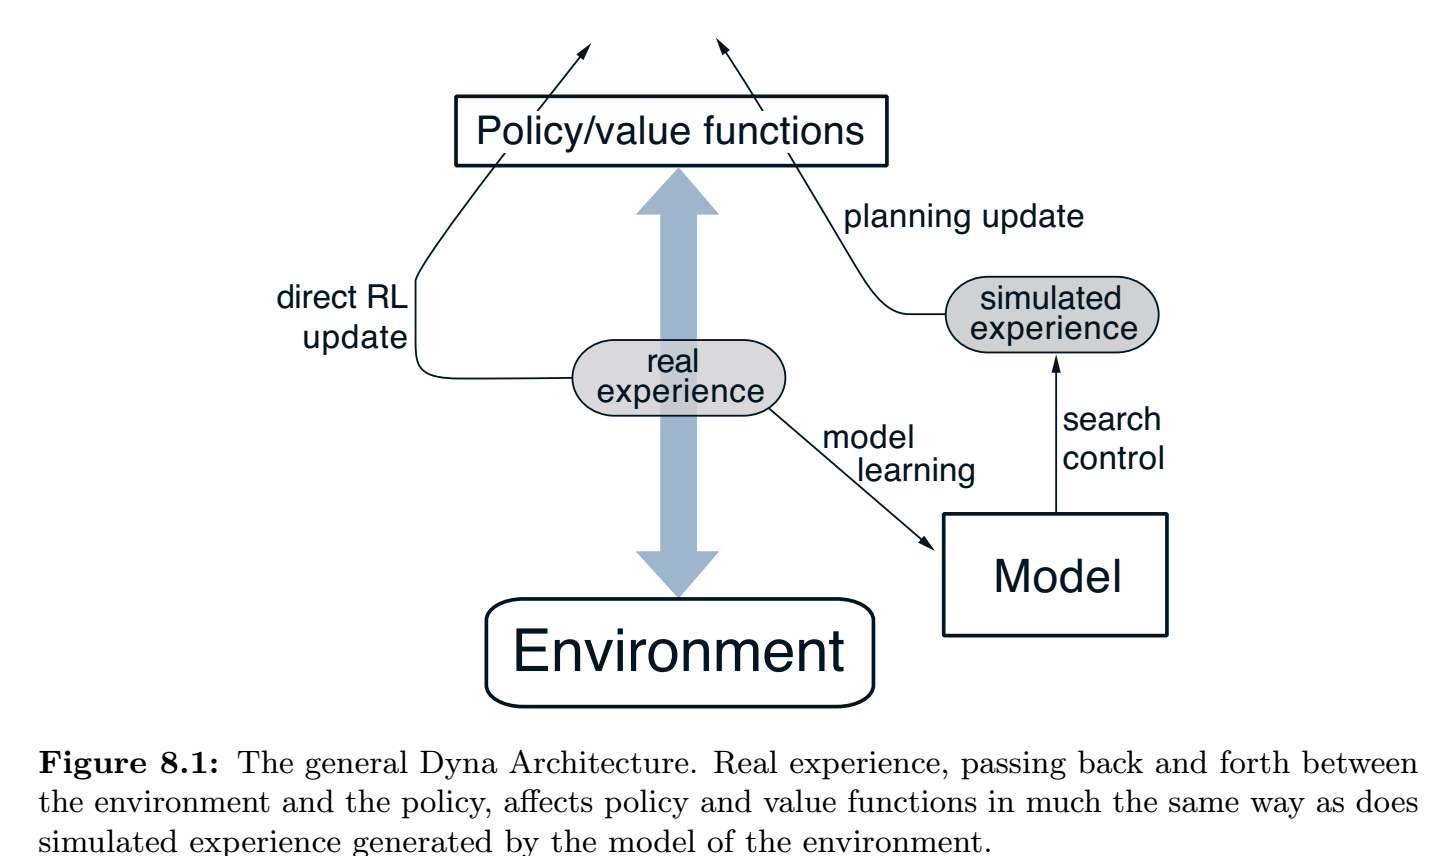
\includegraphics[scale = 0.3]{Dyna_Q.png}}
\end{minipage}
\caption{\footnotesize{\textbf{The Dyna-Q architecture. }}}
\label{fig: Dyna_Q}
\end{figure}
\begin{figure}
\begin{minipage}[t]{1\linewidth}
  \centering
  \centerline{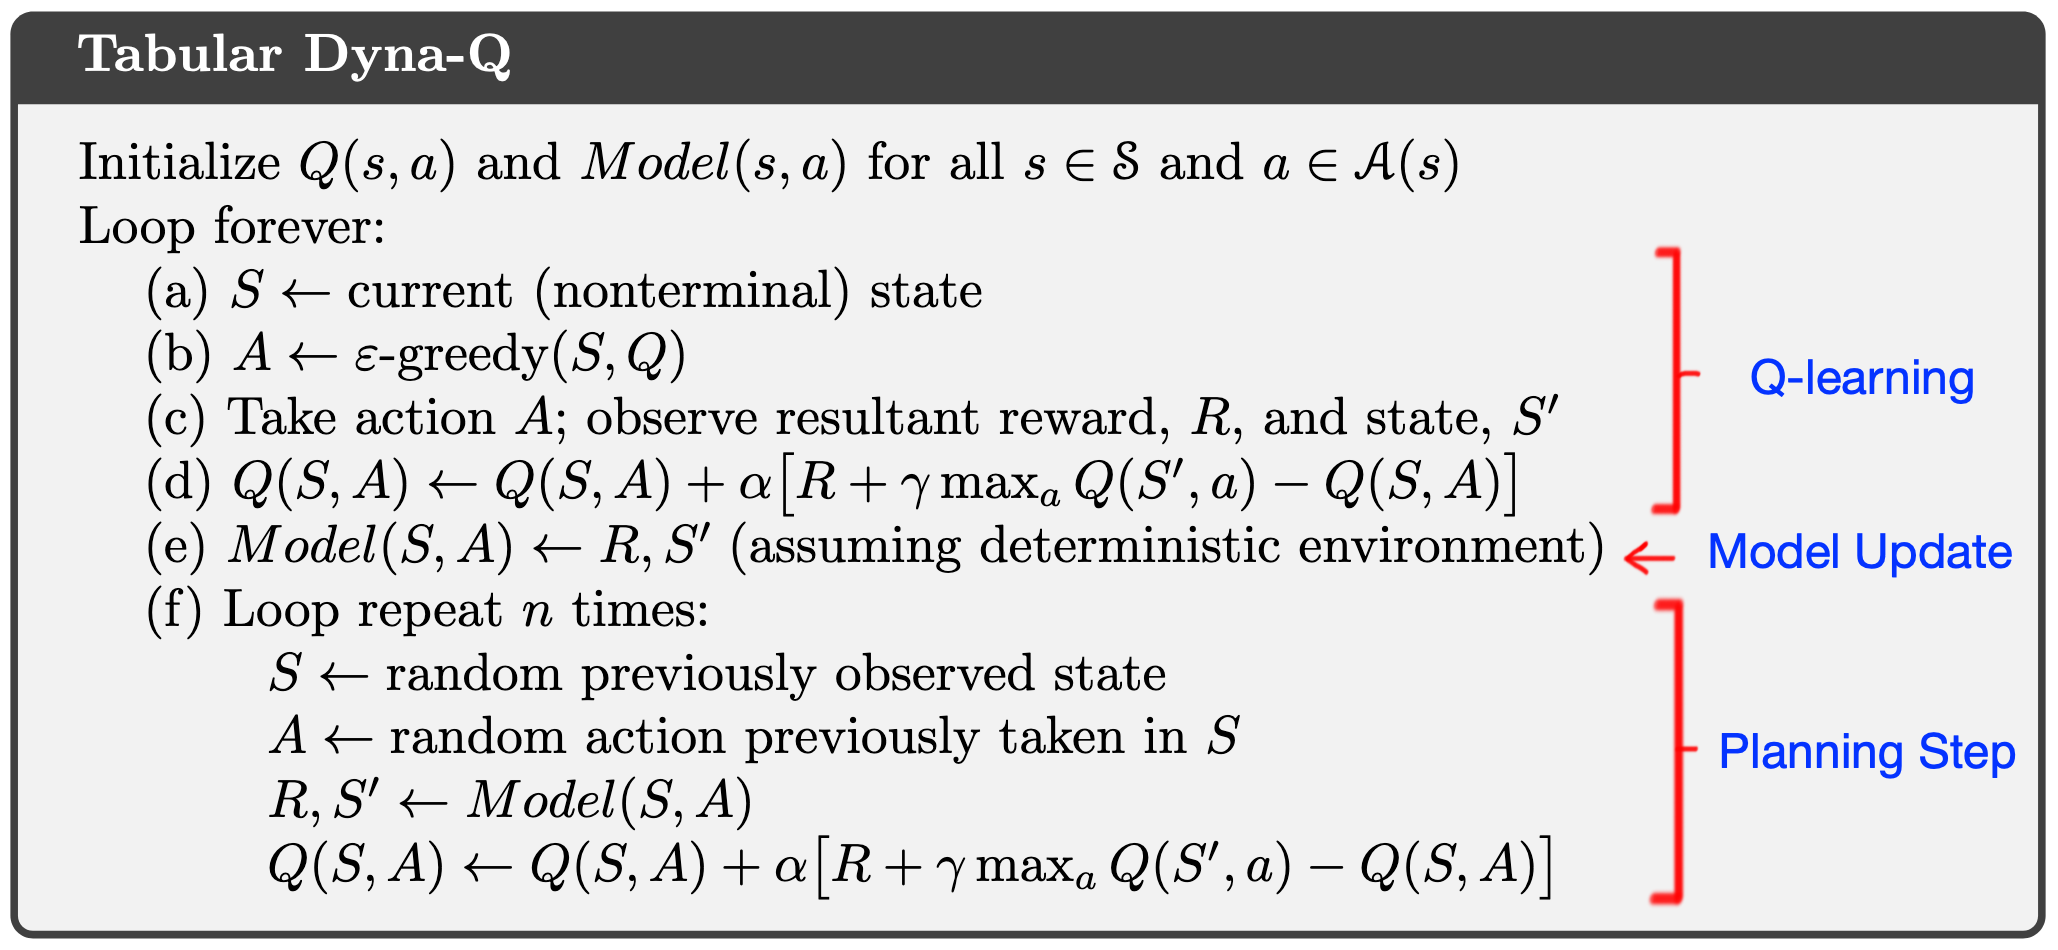
\includegraphics[scale = 0.18]{Tabular_Dyna_Q_alg_notes.png}}
\end{minipage}
\caption{\footnotesize{\textbf{The Tabular Dyna-Q algorithm. }}}
\label{fig: Tabular_Dyna_Q_alg}
\end{figure}

Both direct and indirect methods have \textbf{advantages} and \textbf{disadvantages}. 
\begin{itemize}
\item Indirect methods often make fuller use of a \textbf{limited} amount of experience and thus achieve a better policy with \textbf{fewer environmental interactions}. 

\item Direct methods are much \emph{simpler} and are not affected by \textbf{biases} in the design of the model
\end{itemize} Figure \ref{fig: Dyna_Q} shows the architecture in \textbf{\emph{Dyna-Q}},  an architecture integrating the major functions needed in an \emph{online planning agent}.  It has the following components:
\begin{itemize}
\item \textbf{planning}:  use  random-sample one-step tabular Q-planning method in Figure \ref{fig: tabular_q_planning}. 
\item \textbf{direct RL}:  one-step tabular Q-learning discussed in last chapter. Typically, as in Dyna-Q, the \emph{same} reinforcement learning method is used both for learning from real experience and for planning from simulated experience. The reinforcement learning method is thus the "\emph{final \textbf{common path}}" for both learning and planning.
\item \textbf{model-learning}: \textbf{\emph{table-based}} and assumes the environment is \textbf{\emph{deterministic}}, i.e. given state-action pair, the output of model is \textbf{fixed} reward and next-state pair. It can be coded as \emph{dictionary of dictionaries}. Under this assumption, model learning is simply saving the next state $S_{t+1}$ and reward $R_{t+1}$ for each experienced state $S_{t}$ and action $A_{t}$.
\item \textbf{\emph{search control}}:  the process that selects the \textbf{starting states} and \textbf{actions} for the simulated experiences generated by the model. 

\end{itemize} Figure \ref{fig: Tabular_Dyna_Q_alg} describes the algorithm.  In Dyna-Q, the acting, model-learning, and direct RL processes require little computation, and we assume they consume just a fraction of the time. The remaining time in each step can be devoted to the \emph{planning} process, which is inherently \textbf{computation-intensive}.

In Dyna-Q, learning and planning are accomplished by exactly the same algorithm, operating on real experience for learning and on simulated experience for planning.
Because planning proceeds incrementally, it is trivial to intermix planning and acting. Both proceed as fast as they can. The agent is always \textbf{reactive} and always \textbf{deliberative}, responding \emph{instantly} to the latest sensory information and yet always planning in the background. Also ongoing in the background is the model-learning process. As new information is gained, the model is updated to better \textbf{match reality}. As the model changes, the ongoing planning process will \emph{gradually} compute a different way of behaving to match the new model.

\subsection{When the Model Is Wrong}
Models may be \textbf{incorrect} because the environment is stochastic and only a \emph{limited} number of samples have been observed, or because the model was learned using function approximation that has \textbf{generalized} \textbf{imperfectly}, or simply because the \textbf{environment has changed} and its new behavior has not yet been observed. When the model is incorrect, the planning process is likely to compute a \emph{suboptimal} policy.

The general problem here is another version of the conflict between \textbf{exploration} and \textbf{exploitation}. In a planning context, exploration means trying actions that \emph{\textbf{improve the model}}, whereas exploitation means behaving in the \emph{optimal} way \textbf{given the current model}. We want the agent to explore to find changes in the environment, but not so much that performance is greatly degraded. As in the earlier exploration/exploitation conflict, there probably is no solution that is both perfect and practical, but simple heuristics are often effective.

For example, the \textbf{Dyna-Q+} is an improved version of Dyna-Q with heuristic search.  This agent keeps track for each state–action pair of how many time steps have elapsed since the pair was last tried in a real interaction with the environment, which is denoted as {$\mb{\tau(s, a)}$}. The more time that has elapsed, the greater (we might presume) the chance that the dynamics of this pair has changed and that the model of it is incorrect. During the planning phase, the model uses a special "bonus reward" $=\underline{r+\sqrt{\tau(s, a)}}$ is given on simulated experiences involving the long-untried actions. This encourages the agent to keep testing all accessible state transitions and even to find long sequences of actions in order to carry out such tests.

The Dyna-Q+ agent was changed in two other ways as well. First, actions that \underline{had never been tried} \underline{before} from a state were allowed to be considered in the planning step of the Tabular Dyna-Q algorithm in the box above. Second, the initial model for such actions was that they would \underline{lead back to the same state} with a \underline{reward of zero}.

\subsection{Prioritized Sweeping}
Sometimes, planning can be much more efficient if simulated transitions and updates are focused on particular state–action pairs.  This is called \textbf{Prioritized Sweeping}. The priority is measured according to the size of change for the value estimates when the model updates.

Suppose that the agent discovers a change in the environment and changes its estimated value of one state, either up or down. Typically, this will imply that the values of many other states should also be changed, but the only useful one-step updates are those of actions that lead directly into the one state whose value has been changed. If the values of these actions are updated, then the values of the \textbf{predecessor} states may change in turn. If so, then actions leading into them need to be updated, and
then their predecessor states may have changed. This is called \textbf{backward focusing} of planning computation. 

\section{Summary of all RL methods}
\begin{figure}
\begin{minipage}[t]{1\linewidth}
  \centering
  \centerline{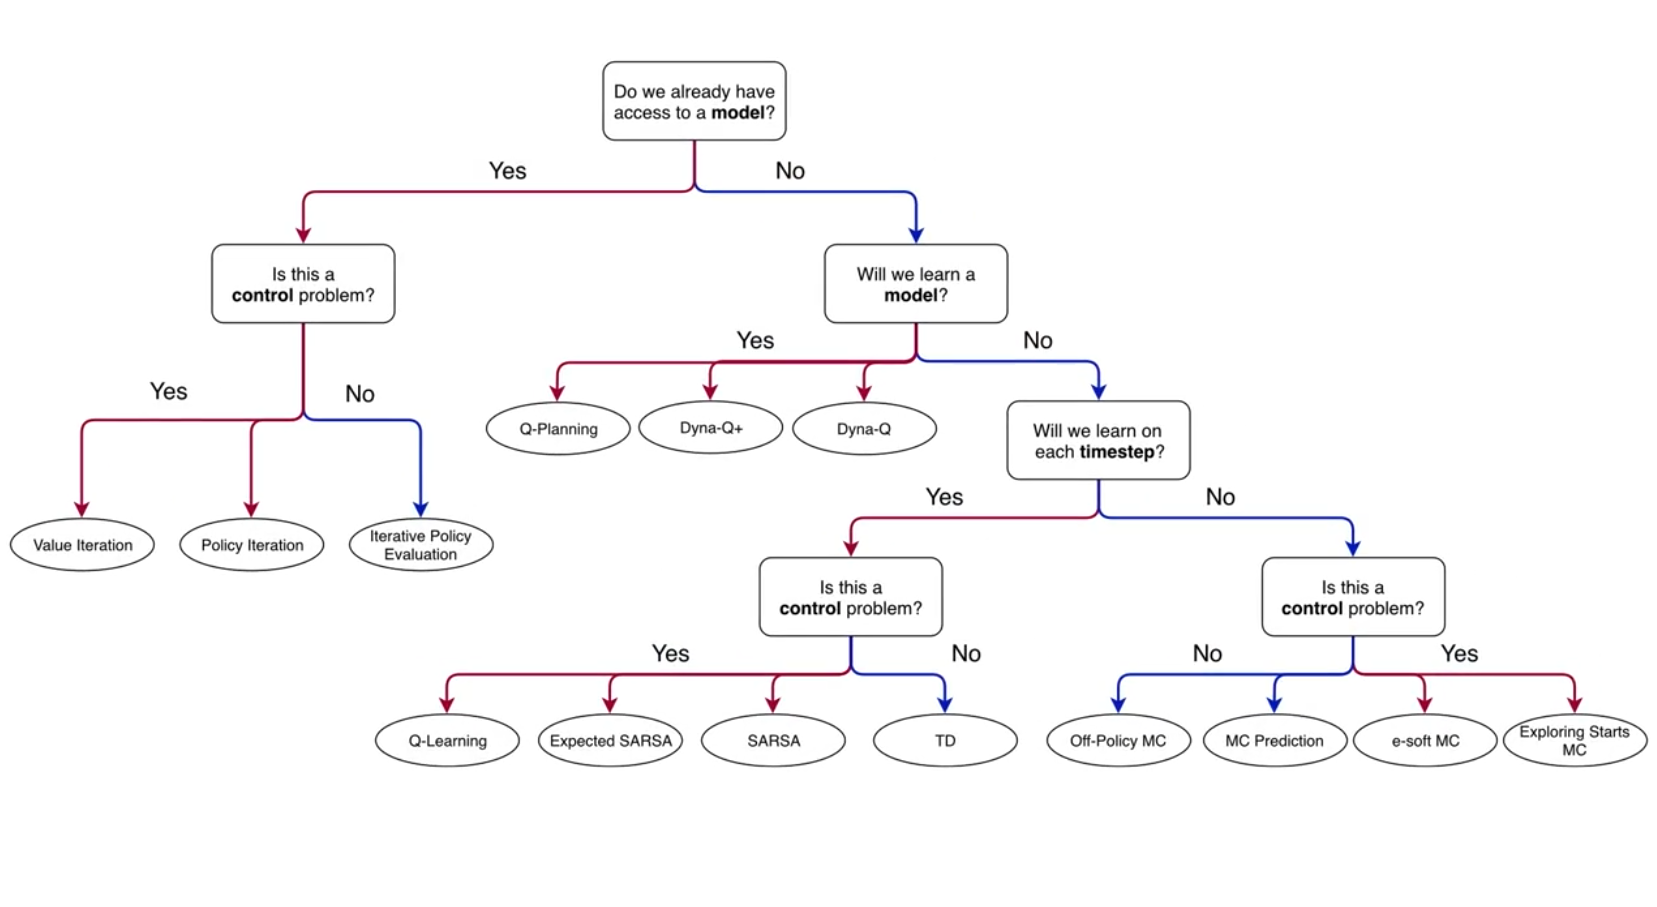
\includegraphics[scale = 0.3]{diagram_tabluar_methods.png}}
\end{minipage}
\caption{\footnotesize{\textbf{Decision-tree to find suitable tabluar methods for reinforcement learning}}}
\label{fig: tabluar_methods_diagram}
\end{figure}
Much of this book has been about different kinds of value-function updates, and we have considered a great many varieties. Focusing for the moment on one-step updates, they vary primarily along three binary dimensions. 
\begin{itemize}
\item update \textbf{state-value}s vs. \textbf{action-value}s: i.e. $v(s)$ or $q(s, a)$
\item estimate the value for the \textbf{optimal policy} vs. for an \textbf{arbitrary given policy}: i.e. $v_{*}(s)$ vs. $v_{\pi}(s)$ or $q_{*}(s,a)$ vs. $q_{\pi}(s,a)$
\item \textbf{expected updates} vs. \textbf{sample updates}: the former considers all possible events that might happen; the later considers a
single sample of what might happen
\end{itemize} Figure \ref{fig: backup_diag_updates} compare their backup diagrams. We can see how DP, MC, TD(0), Sarsa, Q-learning fall into different categories. Dyna-Q uses the Q-learning but it can be replaced by other algorithms in different category since the Dyna architecture is generic and can be applied to other RL algorithm. 

\textbf{Expected updates} yield a better estimate because they are uncorrupted by \textbf{sampling error}, but they also require more computation, and computation is often the limiting resource in planning. To properly assess the relative merits of expected and sample updates for planning we must control for their different \textbf{computational requirements}. This is also determined by the \emph{\textbf{branching factor}}: the number of possible next states with non-zero transition probability. The higher the branching factor, the more computational resources expected updates required compared to sample updates. In a large problem with many state-action pairs, we are often
in the latter situation where the sample update is more feasible. 


The following decision-tree diagram Figure \ref{fig: tabluar_methods_diagram} shows us how to decide which \emph{\textbf{Tabular} RL method} is suitable for our problem. In Tabular RL, the value functions are stored in a table with each state/state-action pair pointing to a real-time value. This is different from Functional Approximation RL methods, which assume that the value function is of some parametric functions. 


According to our knowlege on environment, the RL methods learned before can be categorized as model-based learning and model-free learning
\begin{itemize}
\item \textbf{model-based learning}: as discussed above including the DP method. The followings are incremental updates in policy evalution stage from \textbf{Dynamic Programming} method via Bellman equation or Bellman optimality  equation. The \emph{state-value function} (prediction) \textbf{expected updates} are formulated as below: 
\begin{align*}
v_{\pi}(s) &\leftarrow \sum_{a}\pi(a|s)\sum_{s'}\sum_{r}p(s', r| s, a)\brac{r + \gamma v_{\pi}(s')} \\
&\leftarrow \E{\pi}{R_{t+1}  + \gamma\,v_{\pi}(S_{t+1}) | S_{t} = s} \\
v_{*}(s) &\leftarrow  \max_{a\in \cA(s)}\sum_{s'}\sum_{r}p(s', r|s, a)\brac{r + \gamma v_{*}(s')} \\
&\leftarrow  \max_{a\in \cA(s)}\E{}{R_{t+1} + \gamma v_{*}(S_{t+1}) | S_{t}=s, A_{t}=a}.
\end{align*} Same for  \emph{action-value function} (control), the \emph{expected updates} are as below: 
\begin{align*}
q_{\pi}(s, a) &\leftarrow\sum_{s', r}p(s', r|s,a)\brac{r+ \gamma \sum_{a'}\pi(a'|s')q_{\pi}(s', a')} \\
&\leftarrow \E{}{R_{t+1} + \gamma q_{\pi}(S_{t+1}, A_{t+1}) | S_{t}=s, A_{t}=a}\\
q_{*}(s, a) &\leftarrow  \sum_{s'}\sum_{r}p(s', r|s, a)\brac{r + \gamma  \max_{a'\in \cA(s)}q_{*}(s', a')} \\
&\leftarrow \E{}{R_{t+1} + \gamma \max_{a'\in \cA(s)}q_{*}(S_{t+1}, a') \Big| S_{t}=s, A_{t}=a}.
\end{align*}

\item \textbf{model-free learning}, i.e. sample-based reinforcement learning. We have learned the \textbf{Monte Carlo methods} and the Temporal Difference learning methods.  The incremental \textbf{sample updates} for  Monte Carlo methods in policy evalution stage are formulated as below: 
\begin{align*}
V(S_{t}) &\leftarrow V(S_{t}) + \alpha_{t}\paren{G_{t} - V(S_{t})} \\
Q(S_{t}, A_{t}) &\leftarrow Q(S_{t}, A_{t}) + \alpha_{t}\brac{G_{t}  - Q(S_{t}, A_{t})},
\end{align*} where $G_{t}$ is the sample return accumulated starting at $t+1$ until the end of episode.

On the other hands, the incremental  \textbf{sample updates} update for \textbf{Temporal Difference learning} methods are formulated as follows:  
For state-value function updates (prediction)
\begin{align*}
V(S_{t}) &\leftarrow V(S_{t}) + \alpha_{t}\brac{\hat{G}_{t}  -  V(S_{t})}. \\
 \text{  \textbf{TD(0)} }\quad\hat{G}_{t} &= R_{t+1} + \gamma V(S_{t+1}).
\end{align*} For action-value function (control), the \emph{sample updates} are
\begin{align*}
Q(S_{t}, A_{t}) &\leftarrow Q(S_{t}, A_{t}) + \alpha_{t}\brac{\hat{G}_{t}  - Q(S_{t}, A_{t})}.  \\
 \text{  \textbf{Sarsa} }\quad\hat{G}_{t} &= R_{t+1} + \gamma Q(S_{t+1}, A_{t+1}) \\
\text{  \textbf{Q-Learning} }\quad\hat{G}_{t} &=  R_{t+1} + \gamma \max_{a'\in \cA(S_{t+1})}Q(S_{t+1}, a')  \\
 \text{  \textbf{Expected Sarsa} }\quad\hat{G}_{t} &= R_{t+1} + \gamma\sum_{a'}\pi(a'|S_{t+1})Q(S_{t+1}, a') .
\end{align*} Note that instead of using the sample returns, TD methods use boostrapping to approximate the return based on reward and old estimate of successor states. 
\end{itemize} Figure \ref{fig: backup_diag_updates} shows the back-up update diagrams for all of these methods.  

\begin{figure}
\begin{minipage}[t]{1\linewidth}
  \centering
  \centerline{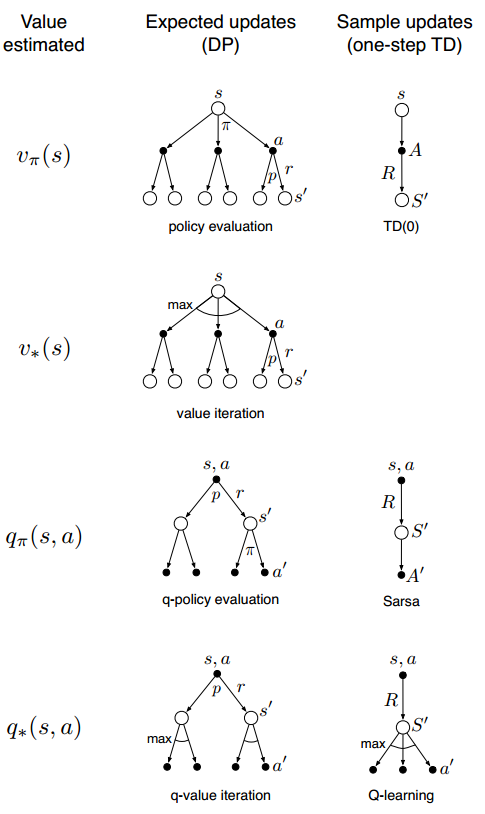
\includegraphics[scale = 0.5]{backup_diag_updates.png}}
\end{minipage}
\caption{\footnotesize{\textbf{A comparison of all RL methods discussed by far. }}}
\label{fig: backup_diag_updates}
\end{figure}

\newpage
\bibliographystyle{plainnat}
\bibliography{reference.bib}
\end{document}